\documentclass[]{elsarticle} %review=doublespace preprint=single 5p=2 column
%%% Begin My package additions %%%%%%%%%%%%%%%%%%%

\usepackage[hyphens]{url}

  \journal{WG-EMM 2021} % Sets Journal name

\usepackage{graphicx}
%%%%%%%%%%%%%%%% end my additions to header

\usepackage[T1]{fontenc}
\usepackage{lmodern}
\usepackage{amssymb,amsmath}
% TODO: Currently lineno needs to be loaded after amsmath because of conflict
% https://github.com/latex-lineno/lineno/issues/5
\usepackage{lineno} % add
\usepackage{ifxetex,ifluatex}
\usepackage{fixltx2e} % provides \textsubscript
% use upquote if available, for straight quotes in verbatim environments
\IfFileExists{upquote.sty}{\usepackage{upquote}}{}
\ifnum 0\ifxetex 1\fi\ifluatex 1\fi=0 % if pdftex
  \usepackage[utf8]{inputenc}
\else % if luatex or xelatex
  \usepackage{fontspec}
  \ifxetex
    \usepackage{xltxtra,xunicode}
  \fi
  \defaultfontfeatures{Mapping=tex-text,Scale=MatchLowercase}
  \newcommand{\euro}{€}
\fi
% use microtype if available
\IfFileExists{microtype.sty}{\usepackage{microtype}}{}
\usepackage[]{natbib}
\bibliographystyle{plainnat}

\ifxetex
  \usepackage[setpagesize=false, % page size defined by xetex
              unicode=false, % unicode breaks when used with xetex
              xetex]{hyperref}
\else
  \usepackage[unicode=true]{hyperref}
\fi
\hypersetup{breaklinks=true,
            bookmarks=true,
            pdfauthor={},
            pdftitle={A preliminary evaluation of the evidence supporting fishery-driven localised depletion effects on the performance and demographic trends of pygoscelid penguins in Subarea 48.1},
            colorlinks=false,
            urlcolor=blue,
            linkcolor=magenta,
            pdfborder={0 0 0}}
% For pandoc feature
\ifLuaTeX
  \usepackage{luacolor}
  \usepackage[soul]{lua-ul}
\else
  \usepackage{soul}
\fi

\setcounter{secnumdepth}{0}
% Pandoc toggle for numbering sections (defaults to be off)
\setcounter{secnumdepth}{0}


% tightlist command for lists without linebreak
\providecommand{\tightlist}{%
  \setlength{\itemsep}{0pt}\setlength{\parskip}{0pt}}

% From pandoc table feature
\usepackage{longtable,booktabs,array}
\usepackage{calc} % for calculating minipage widths
% Correct order of tables after \paragraph or \subparagraph
\usepackage{etoolbox}
\makeatletter
\patchcmd\longtable{\par}{\if@noskipsec\mbox{}\fi\par}{}{}
\makeatother
% Allow footnotes in longtable head/foot
\IfFileExists{footnotehyper.sty}{\usepackage{footnotehyper}}{\usepackage{footnote}}
\makesavenoteenv{longtable}



\usepackage{float} \floatplacement{figure}{H}
\usepackage{booktabs}
\usepackage{longtable}
\usepackage{array}
\usepackage{multirow}
\usepackage{wrapfig}
\usepackage{float}
\usepackage{colortbl}
\usepackage{pdflscape}
\usepackage{tabu}
\usepackage{threeparttable}
\usepackage{threeparttablex}
\usepackage[normalem]{ulem}
\usepackage{makecell}
\usepackage{xcolor}



\begin{document}


\begin{frontmatter}

  \title{A preliminary evaluation of the evidence supporting
fishery-driven localised depletion effects on the performance and
demographic trends of pygoscelid penguins in Subarea 48.1}
    \author[Norwegian Polar Institute, Tromsø, Norway]{Andrew Lowther%
  %
  }
   \ead{andrew.lowther@npolar.no} 
    \author[Institute of Marine Research, Tromsø, Norway]{Martin Biuw%
  %
  }
   \ead{martin.biuw@hi.no} 
    \author[Institute of Marine Research, Tromsø, Norway]{Ulf Lindstrøm%
  %
  }
   \ead{ulf.lindstroem@hi.no} 
    \author[Institute of Marine Research, Bergen, Norway]{Bjørn Krafft%
  %
  }
   \ead{bjorn.krafft@hi.no} 
      \cortext[cor1]{Corresponding author}
  
  \begin{abstract}
  Two independent lines of evidence have been presented to the working
  groups and SC-CAMLR that claim to demonstrate that fishery-driven
  localised depletion of krill around pygoscelid penguin colonies has
  had a deleterious effect on their performance traits and demographic
  trends, that are equivalent to the impacts of climate variation. One
  study utilises 30 years of penguin foraging and reproductive
  performance measurements collected at two colonies in the South
  Shetland Islands while the other uses demographic rate changes derived
  from a comprehensive dataset of penguin population count data across
  Subarea 48.1 matched against acoustic measurements of krill biomass
  and krill catches at the gSSMU scale \citep{Watters2020}. The second
  uses estimated population trajectories across a wide range of penguin
  breeding colonies alongisde krill catches within 30km
  \citep{Kruger2021}. Both studies then explore the synergistic
  relationships to measurements of broad-scale climactic variation (El
  Nino Southern Oscillation; ENSO, and the Southern Annular Mode; SAM).
  Herein we provide a preliminary assessment of the efficacy of both
  approaches in drawing conclusions, that are now being used at the
  Commission level, as representing sound scientific advice. We
  demonstrate that several underlying assumptions in Watters et al.~2020
  are contrary to the published scientific literature, and when the
  model syntax is re-written to reflect this, predicted penguin
  performance against long term expected means are substantially
  different to those presented to CCAMLR. \emph{STUFF ON KRUGER} needed
  here. While our preliminary assessment focuses on potential issues,
  future work will centre on considering competitive interactions both
  at appropriate time and space scales between the fishery as well as
  between a range of krill dependent predators beyond just pygoscelid
  penguins.
  \end{abstract}
  
 \end{frontmatter}

\section{Introduction}\label{introduction}

Concerns over the potential impact of localised depletion of krill
through concentrated fishing effort on krill-dependent predators has
been a topic of debate within SC-CAMLR and its Working Groups for many
years (REF). Recently, two studies have been presented that suggest that
local harvesting rates can impact predator performance to the same
degree as poor environmental conditions \citep{Watters2020}, and that
synergistic impacts on predators are evident when poor climactic
conditions are coupled with locally high harvest rates
\citep{Kruger2021}.

While both studies attempt to tackle the same overall problem, they do
so using very different methodologies. \citet{Watters2020} exploit a
considerable dataset; a substantial multi-species time series of
\textbf{\emph{a large number of}} penguin performance indices (including
those collected under CEMP) collected over three decades at two sites
(Cape Shireff on Livingstone Island and Copacabana on King George
Island, South Shetland Islands; Figure 1) and more than a decade of
summer acoustic \textbf{\emph{krill}} surveys that cover the at-sea
distributions of Chinstrap, gentoo and Adélie penguins. Drawing in
monthly krill catch statistics from the C1 Catch and Effort dataset and
climactic data (Oceanic Niño Index; ONI), the authors use a hierarchical
analysis of variance approach to estimate the variance in performance
indices as a function of Local Krill Biomass (LKB), Local Harvesting
Rates (LHR; the ratio of krill catch to LKB) and ONI. In contrast,
\citet{Kruger2021} utilise a broader range of penguin colonies across
the same three species throughout the Antarctic Peninsula area, in
combination with their respective abundance survey estimates
\textbf{\emph{(number of occupied nests)}} from an open-source database
(www.penguinmap.org). The authors calculate population trends for
appropriate sites, and \textbf{\emph{\st{using}}} \textbf{\emph{use}}
the CCAMLR C1 Catch and Effort data to extract annual catch values
within a 30km radius of each colony. Finally, \citet{Kruger2021} use the
\textbf{\emph{\st{trajectory of the trend (positive; increase versus
negative; decrease)}}} \textbf{\emph{sign of the difference in number of
nests between annual surveys}} as a response in a binomial generalised
linear mixed \textbf{\emph{effects}} model using the
\textbf{\emph{\st{summed}}} \textbf{\emph{accumulated}} annual
catch\textbf{\emph{\st{, a lagged trend of the}}} \textbf{\emph{and mean
wintertime}} Southern Annular Mode \textbf{\emph{(SAM)}}
\textbf{\emph{\st{and the SOMETHING ON ONI ????}}} to determine the
relative contributions of each predictor and their interactive effects
on population abundance trends. Both studies draw similar conclusions;
that local harvesting levels of krill impact predators, and the degree
of impact can either be similar to that of poor environmental conditions
or have a synergistic impact when high local harvesting coincides with
poor conditions.

These conclusions have been propagated into Commission documentation
supporting the reformulation of the D1MPA proposal (CCAMLR-39/BG/02) as
well as into Commission discussions (CCAMLR-39, Para 5.48 \& Para 5.51).
However, while the two studies have moved from Working Papers of EMM
into the realms of the peer-reviewed literature, \textbf{\emph{\st{we
have}}} \textbf{\emph{there are}} some areas of concern
\textbf{\emph{\st{about}}} \textbf{\emph{regarding}} the structuring of
these studies that we \textbf{\emph{\st{feel warrant raising}}}
\textbf{\emph{think deserve some extra attention}}.
\textbf{\emph{\st{Our preliminary review raises}}} \textbf{\emph{Some of
these}} concerns \textbf{\emph{are}} unique to each study
\textbf{\emph{\st{but also}}} \textbf{\emph{while others are}} common
across both, and we structure our paper accordingly. Firstly, we review
\citet{Watters2020} and \citet{Kruger2021} through the lens of some of
the ecological assumptions made versus the available evidence pertaining
to them. Within the constraints of the data and analytical methods that
are available from the studies, we also quantify how rationalising these
assumptions to the evidence available impacts on the conclusions drawn.
We then highlight some overarching concerns applicable to both papers.

\section{\texorpdfstring{\citet{Watters2020} / WG-EMM
2019/11}{@Watters2020 / WG-EMM 2019/11}}\label{watters2020-wg-emm-201911}

A key goal for the paper is to highlight the mismatch between the areal
scales of fisheries management and ecological \textbf{\emph{\st{the}}}
interactions between fishing extractions and dependent predators. To do
this, the authors create two strata aligned with groups of SSMU (gSSMU);
gSSMU \#1 including those SSMU inside the Bransfield Strait (APBSE and
APBSW and gSSMU \#2 incorporating SSMU north of the South Shetlands,
including Elephant Island (APDPE, APDPW and APEI) represented in Figure
1. These gSSMU cover \(15,500nm^2\) and \(20,600nm^2\), respectively,
and are used to characterise both krill biomass and harvesting rates
that are ``local'' to the penguin colonies for which performance data
are used. The reasoning behind scaling to gSSMU are linked to the
foraging behaviour of the penguins for which performance data area
available i.e.~breeding, adult pygoscelids. The authors cite
\citet{Hinke2017} as the evidence supporting usage of the two gSSMU as
appropriate strata.

Pygoscelid penguins exhibit staggered breeding, with Adélies commencing
first, followed by chinstraps then gentoos \citep{Black2016}. Adélie
penguins are the first to fledge their chicks and thus cease to be
centrally foraging, typically departing mid-February for their moulting
grounds on the sea ice. Chinstrap penguins depart for a pre-moult
foraging trip towards the end of February and return to land in order to
moult, before departing again for their overwinter trip
(\citet{Hinke2015}; \citet{Hinke2019}; Figure 2). Conversely, Gentoo
penguins appear to remain in close proximity to their breeding colonies
overwinter .

We use the Argos-CLS PTT telemetry data provided by the supporting
studies to characterise the actual at-sea habitat used, in the context
of the relative stage of breeding for each species. For each species, we
refrain from undertaking extensive state-space modelling of location
errors and merely exclude locations with a ``Z'' error class, then
calculated the 99\% Minimum Convex Polygon (home range) and their
associated areas in \(nm^2\). For chinstrap penguins at Cape Shireff,
this equated to a home range area of \textasciitilde{}\(4,782nm^2\), or
only 23\% of the gSSMU to which their performance metrics are indexed
against \citep{Watters2020}. For the same species at Copacobana the 99\%
MCP home range is 2,905\(nm^2\), or \textasciitilde19\% of gSSMU 1 in
the Bransfield Strait. Similarly for Adélie penguins, the breeding
foraging range occupied 1,139\(nm^2\) or only \textasciitilde7\% of the
area of gSSMU \#1. After breeding, available overwinter PTT telemetry
and light geolocating data on chinstrap and Adélie penguins suggests a
wide dispersal westwards into the Pacific sector of the Southern Ocean,
and eastwards into the Weddell Sea and Atlantic sectors, with a
relatively small proportion of chinstraps from the study sites remaining
within 500km of their breeding colonies \citep{Hinke2019}. Yet despite
the evidence supporting widescale post-breeding migration of both Adélie
and Chinstrap penguins, the model used by \citet{Watters2020} constrains
both species from Copacobana to gSSMU 1 and Chinstraps from Cape Shireff
to gSSMU 2 over winter (\citet{Watters2020}; Supplementary Material 1 \&
2, code lines 258 to 259). This has the effect of constraining the
variability in performance indices from these species to LHR, LKB and
ONI over winter in areas where the species has a demonstrated tendency
to migrate away from. This is particularly important given that the
fishery can now be characterised with a late autumn/early winter start
which places a seasonal element on LHR towards increased values in the
winter (Figure 4).

Our preliminary review thus far raises two areas of concern. Firstly,
that the scales at which ``local'' predictors are summarised are in some
cases five times larger than the habitat exploited by the penguins
monitored. Secondly, that the known overwinter migratory behaviour of
Adélie and Chinstrap penguins are poorly reflected in the model
formulation. To demonstrate the impact that these ecological assumptions
have on the model output, we rerun the model of \citet{Watters2020} with
modified code. To avoid an overly burdensome paper, we shortly summarise
those code changes here, and if requested during the meeting we are
happy to include the rmarkdown version of this paper with the modified
code in place, or submit the modifications to the meeting in some other
format.

We also note an additional coding error that may influence how the
original (i.e.~unmodified) results are interpreted. In summarising the
model outputs into boxplots, the code relating to developing Figure 2
(Supplementary Material 1, lines 661-665) seemingly classifies the
``Worst Case'' (\({-0.5}\) \(^{\circ}\)C \textless{} ONI \textless{} 0.5
\(^{\circ}\)C; LKB \textgreater{} 1 Mt; and LHR \(\geqslant\) 0.1) using
column 36 from the output dataframe, which actually reflects ``ONI
\textgreater{} 0.5 \(^{\circ}\)C; LKB \textgreater{} 1 Mt; and LHR
\(\geqslant\) 0.1'' - that is, in the ``Worst Case'', ONI is in its
``warm'' phase as opposed to ``neutral''. We thus relabel the output
boxplot axes labelling to reflect the conditions representing ``worst
case'' accordingly.\\
\newline \emph{modifications}

\begin{enumerate}
\def\labelenumi{\arabic{enumi}.}
\tightlist
\item
  We scale the gSSMU LKB to the SSMU that the summer tracking data
  indicate penguins occupied. For example, we scale LKB for Cape Shireff
  chinstrap penguins solely to ADPDW by multiplying the gSSMU LKB by the
  areal ratio of ADPDW/gSSMU \#2. We then select the corresponding SSMU
  catch values provided in \citet{Watters2020} to estimate SSMU-scale
  LHR.
\item
  We remove Adélie and Chinstrap penguins from the model formulation
  over winter; that is, we attribute each species as ``NA'' during
  winter, to account for dsipersal after breeding.\\
\item
  The authors place LKB/LHR values in March into the ``summer'' period.
  However fishing effort over the period that performance indices are
  available is not uniform over the thirty year period, with catch over
  the preceding decade showing a nonlinear increase from the middle of
  March and three years where catch rates increased rapidly from the
  beginning of the month (Figure 4). Given the highly variable rates of
  catch throughout the study period, we run scenarios that classify
  March as either summer or winter to reflect the linkage between March
  and the breeding state of penguins i.e.~Adélie and Chinstrap penguins
  have either migrated out of the area or have ceased to be centrally
  foraging species by March.
\end{enumerate}

We run a total of six permutations of the modifications, grouped into
three pairs, as follows:

\begin{enumerate}
\def\labelenumi{\arabic{enumi}.}
\tightlist
\item
  Performance indices from all species, using estimates of LKB and LHR
  at the SSMU level, considering March either in a) summer or b) winter.
  (Areal scaling down of gSSMU LKB and using SSMU scale C1 monthly
  aggregated catch data).
\item
  Performance indices from Adélie and Chinstrap penguins, matched at the
  SSMU level with March either in a) summer or b) winter
\item
  Performance indices from Gentoo penguins matched at the SSMU level
  with March either in a) summer or b) winter.
\end{enumerate}

We present the outputs both in the same boxplot format as Figure 2 in
the original manuscript, and as individual cases grouped and
colour-coded as ONI ``warm / \(\geqslant\) 0.5'' (red), ONI ``neutral /
-0.5 \textless\textgreater{} +0.5'' (white) and ONI ``cold / \textless{}
-0.5'' (blue). \textbf{\emph{These symbols look a bit weird. What did
you intend to write?}} \newline   \newline   \emph{results}\\
\newline

\section{\texorpdfstring{\citet{Kruger2021} / WG-EMM
2019/10}{@Kruger2021 / WG-EMM 2019/10}}\label{kruger2021-wg-emm-201910}

The key objective of the paper by \citet{Kruger2021} is to examine the
potential synergistic effects of climate change and increased fishing
activity in recent decades on the breeding performance of chinstrap and
gentoo penguins. The authors make the implicit assumption that there has
been a general decrease in krill density in response to climate change,
although this is still a topic of debate and is not supported by recent
large-scale surveys in the Scotia Sea (REF 2019 Krill survey report).

\textbf{\emph{Perhaps describe the model already here, to set the scene
for the data input issues?}}

To address this topic, the authors use data on the number of occupied
nests (breeding pairs) counted at a large number of sites throughout the
Antarctic Peninsula between 1980 and 2017. These data are available from
the Mapping Application for Penguin Populations and Projected Dynamics
(MAPPPD) data archive (REF to website and Humphries et al.~2017).
\citet{Kruger2021} include count data on occupied nests based on surveys
carried out in November or December, reflecting the early breeding
season. They further subset the data to include only colonies for which
at least 2 survey estimates are available throughout the 38-year period
under consideration (i.e.~1980-2017). These data are provided in the
supplementary materials for the paper. Based on the raw counts, they
calculate an index of temporal variation in population growth rate
using: \[\lambda_{std}=((n_b/n_a)/years_{b-a}-1\] where \(n\) is the
number of breeding pairs counted in Nov-Dec of a given year, \(b\) and
the number of breeding pairs counted in the nearest previous year \(a\)
in which a Nov-Dec survey was conducted, divided by the interval between
surveys (i.e.~\(b-a\)). While this index may be a robust index of
population change, the authors then convert \(\lambda_{std}\) into a
binary index, \(bin\lambda_{std}\) that takes the value 1 for negative
growth and 0 for positive growth. The rationale is that this value can
be interpreted as the probability of population decline in response to
catch and environmental change, but it also completely ignores how the
absolute or relative change in population size may respond to fisheries
and environmental change.

Another problem with this index is the interval between consecutive
surveys. Based on the \citet{Kruger2021} supplementary dataset,
intervals between surveys exceeding one year are relatively common
(intervals \textgreater1 year: 27\% for Chinstraps and 48\% for Gentoos;
intervals \textgreater2 years: 17\% for Chinstraps and 15\% for Gentoos,
Table 1). As we describe below, these larger intervals may represent a
temporal mismatch problem, given the fact that response variables only
represent conditions within one year prior to the breeding season.

As in the case of \citet{Watters2020}, \citet{Kruger2021} also use
CCAMLR C1 fisheries data to estimate fishing pressure, but in this case
only hauls within a 30km radius are considered for each specific colony.
This selection is based previous observations that foraging of
pygoscelid penguins is more probable within 30 km of the colonies during
the breeding season \textbf{\emph{refer to Warwick-Evans et al.~2018}}.
While they initially summarise these data within distinct time periods,
reflecting different important stages of the penguin annual cycle, these
are only used for illustrative purposes \citep[Fig 3 in][]{Kruger2021}.
However, when modelling the effect of fisheries on population response,
the authors use accumulated annual catches within these 30km areas,
thereby making the assumption that penguin breeding performance is
affected by resource availability in the immediate vicinity of their
specific breeding colonies also during the non-breeding period in
winter. While this might be valid for gentoo penguins which appear to
remain close to the breeding colonies also outside the breeding season,
it is questionable how appropriate this is for chinstraps that disperse
much more widely during winter (see above). This spatio-temporal
mismatch problem is further exacerbated in cases where intervals between
consecutive breeding population surveys exceed one year.

The authors use monthly data on the Southern Annular Mode (SAM) index
\textbf{\emph{refer to Kwok and Comiso 2002; Doddridge and Marshall
2017}} to represent environmental variability. Based on an observed 0-3
month lagged correlation between SAM and relevant local climate
variables (fractional sea ice cover, open water sensible heat flux and
sea level air pressure), the authors exclude SAM values for months
coinciding with the breeding season.

To test statistically the effects of local fishing pressure and
environmental conditions on penguin breeding performance,
\citet{Kruger2021} fit a binomial Generalized Linear Mixed Effects model
of the form: \[bin\lambda_{std}=catch_y*SAM+(1|colony\text{ }ID)\]

where \(catch_y\) is the accumulated krill catch within 30km of each
colony during the year immediately leading up to the second survey in an
interval (i.e.~equivalent to \(year_b\) in the population growth rate
equation above), SAM is the SAM index during the winter prior to the
same survey (i.e.~temporally overlapping with most of the catch data
accumulation period). the term in brackets indicate a random intercept
effect on colony. Unlike in the case of the \citet{Watters2020} paper,
scripts are not provided for the analyses done by \citet{Kruger2021},
and therefore we have not been able to recreate their analyses exactly
and test various aspects of data input, underlying assumptions and
alternative model formulations.

NEEDS WORKING ON - A LOT :) BULLET POINTS FROM THE GOOGLE DOC BELOW:

\begin{enumerate}
\def\labelenumi{\arabic{enumi}.}
\tightlist
\item
  Contention that population trends (rate of growth/decline) are related
  to synergistic impacts of climate change and localized fishing
  pressure
\item
  Autumn/winter SAM is an appropriate proxy for krill abundance (i.e no
  consideration of interactive effects between SAM and ONI)
\item
  The validity of linear interpolation across multiple years
  (\textgreater1) has not been analysed.
\item
  30km buffer around colonies to extract fishing effort is appropriate
  over winter
\item
  Using population rates calculated between survey efforts sometimes
  several years apart are appropriate
\item
  Assumption that calculated population rates directly reflect
  mortalities \textbf{\emph{This one I don't understand. I don't think
  their assumption actually is that the rate reflects mortality, only
  that it reflects changes in the number of birds returning to breed
  (irrespective of if they're still alive or not).}}
\item
  No consideration of lagged recruitment (fledging to reproductive age)
  nor ability to detect lagged recruitment with irregular surveying
  effort / lack of banding
\end{enumerate}

AND BELOW ARE POINTS FROM THE HTML WORKING DOCUMENT:

\textbf{Problem 1: There's clearly some discrepancies in amounts of data
here that we may need to approach the authors about.}

\textbf{Problem 2: How representative is this rate value for a specific
year, in the cases where it has been calcluated as a linear change over
a period of several years between surveys?}

\textbf{Problem 3: Is it appropriate to use annually accumulated catch
as an explanatory variable to explain number of breeding pairs observed
in Nov-Dec?}

\textbf{Problem 4: In the case of gentoos, half of the sites never have
positive catch rates within 30 km, while for chinstraps the situation is
not so bad. How does this explain the model fits and conclusions of
Kruger et al.?}

\textbf{Problem 5: If no other climate variables are included in the
model, does their argument really make sense? Why exclude SAM during the
breeding period?}

\textbf{Problem 6. According to the documentation ,this package only
appears to have the capacity to fit a simple LMME, which does not allow
for a binomial response}

\section{Discussion}\label{discussion}

Our preliminary review of the evidence supporting localised effects of
fishing coupled with broad-scale climactic phenomena having an impact on
the vital statistics of pygoscelid penguins (performance and demographic
trends) are based on assumptions that potentially do not reflect current
knowledge of penguin breeding phenology and movement.\\
\newline \emph{DESCRIPTION OF x6 SCENARIOS RUN WITH STIG}\\
\newline   Of greatest concern, however, is that the interpretation of
model outputs from both approaches (either from the original studies or
the modified parameters we describe) are under boundary conditions that
we feel are not appropriate. Both approaches consider only the fishery
and broad-scale climate phenomena as the only two causes of krill
abundance variability at geographic scales relevant to penguins. Neither
study considers, for example, the impact of rebounding baleen whale
populations or migratory male Antarctic fur seals beyond brief
mentioning. Both taxa have increased in abundance throughout the life of
the krill fishery, and there are sufficient telemetry and distance
sampling studies in the scientific literature to demonstrate the degree
and significance of spatiotemporal overlap with breeding penguin
populations (see \citet{Santora2013}, \citet{Lowther2020}, and
Oosthuizen et al., Johannessen et al.~and Lowther et al.~submitted to
this meeting, and Figure 3 as examples). Importantly, the distribution
of these and numerous other unconsidered competitors is not uniform in
either space or time and their impact on local availability of krill is
likely to be considerable.

Similarly, the utilisation of broad-scale climatological phenomena to
characterise impacts at scales that predators are dependent upon is
problematic. The Amundsen Sea Low (ASL) is the dominant climate feature
for the western Antarctic Peninsula. The El Niño Southern Oscillation
(ENSO) modulates the the ASL, with El Niño (La Niña) shallowing
(deepening) its pressure, causing more northwesterly (southeasterly)
winds and upwelling (restricted influx) of Circumpolar Deep Water onto
the shelf. The Southern Annular Mode also influences the pressure of the
ASL, with the current trend of negative SAM constructively
(destructively) interfering with ASL when in phase with El Niño (La
Niña) events (e.g. \citet{Clem2016}). The result is a set of
above-surface climate conditions that drive changes in water mass
intrusion that are dependent on interactions between two climate
processes. However the bathymetry of the Antarctic Peninsula is complex
(particularly at scales that are important to centrally-foraging
predators such as penguins) and the structuring of krill aggregations in
time and space in the WAP have been linked to mesoscale circulation
processes \citep{santoraKrillSpaceComparative2012}, which are unlikely
to be uniformly affected by macroscale processes.

Our work into the future will progress along three lines, and we welcome
any and all offers of collaboration into this work. Firstly, we will
progress this debate into the scientific literature in order to ensure a
balanced discussion occurs in that forum. Secondly, we will be examining
in further detail some of the additional predictors used and their
efficacy, the modelling frameworks into which they are brought, and how
their incorporation influences the interpretation of the responses.
Finally, we shall also be exploring alternative modelling approaches
that reflect more of the physical and biological complexity of the
system in question. In all cases, our goal is to ensure that the best
available objective scientific evidence is presented to our
environmental managers and, where appropriate, flag that disagreement
exists. Our paper should be viewed in this light to generate
constructive dialogue that addresses our common concern of the potential
for localised fishing to impact dependent aspects of the ecosystem.\\
\newpage

\section{Citations}\label{citations}

\newpage

\section{Tables}\label{tables}

\begin{longtable}[]{@{}
  >{\centering\arraybackslash}p{(\linewidth - 4\tabcolsep) * \real{0.2222}}
  >{\centering\arraybackslash}p{(\linewidth - 4\tabcolsep) * \real{0.1667}}
  >{\centering\arraybackslash}p{(\linewidth - 4\tabcolsep) * \real{0.1250}}@{}}
\caption{Frequency distribution (percent) of intervals between
consecutive breeding surveys for chinstrap and gentoo penguins used by
\citet{Kruger2021}.}\tabularnewline
\toprule\noalign{}
\begin{minipage}[b]{\linewidth}\centering
~
\end{minipage} & \begin{minipage}[b]{\linewidth}\centering
Chinstrap
\end{minipage} & \begin{minipage}[b]{\linewidth}\centering
Gentoo
\end{minipage} \\
\midrule\noalign{}
\endfirsthead
\toprule\noalign{}
\begin{minipage}[b]{\linewidth}\centering
~
\end{minipage} & \begin{minipage}[b]{\linewidth}\centering
Chinstrap
\end{minipage} & \begin{minipage}[b]{\linewidth}\centering
Gentoo
\end{minipage} \\
\midrule\noalign{}
\endhead
\bottomrule\noalign{}
\endlastfoot
\textbf{1 year} & 63.03 & 68.29 \\
\textbf{\textgreater1 year} & 26.75 & 48.28 \\
\textbf{\textgreater2 years} & 16.51 & 14.67 \\
\textbf{\textgreater3 years} & 8.95 & 9.3 \\
\textbf{\textgreater4 years} & 7 & 4.26 \\
\textbf{\textgreater5 years} & 3.64 & 3.28 \\
\textbf{\textgreater6 years} & 3.15 & 2.44 \\
\textbf{\textgreater7 years} & 2.31 & 0.98 \\
\textbf{\textgreater8 years} & 1.82 & 0.98 \\
\textbf{\textgreater9 years} & 1.82 & 0.49 \\
\textbf{\textgreater14 years} & 1.33 & 0.49 \\
\textbf{\textgreater15 years} & 1.33 & 0 \\
\textbf{\textgreater19 years} & 0.84 & 0 \\
\end{longtable}

\section{Figures}\label{figures}

\begin{figure}
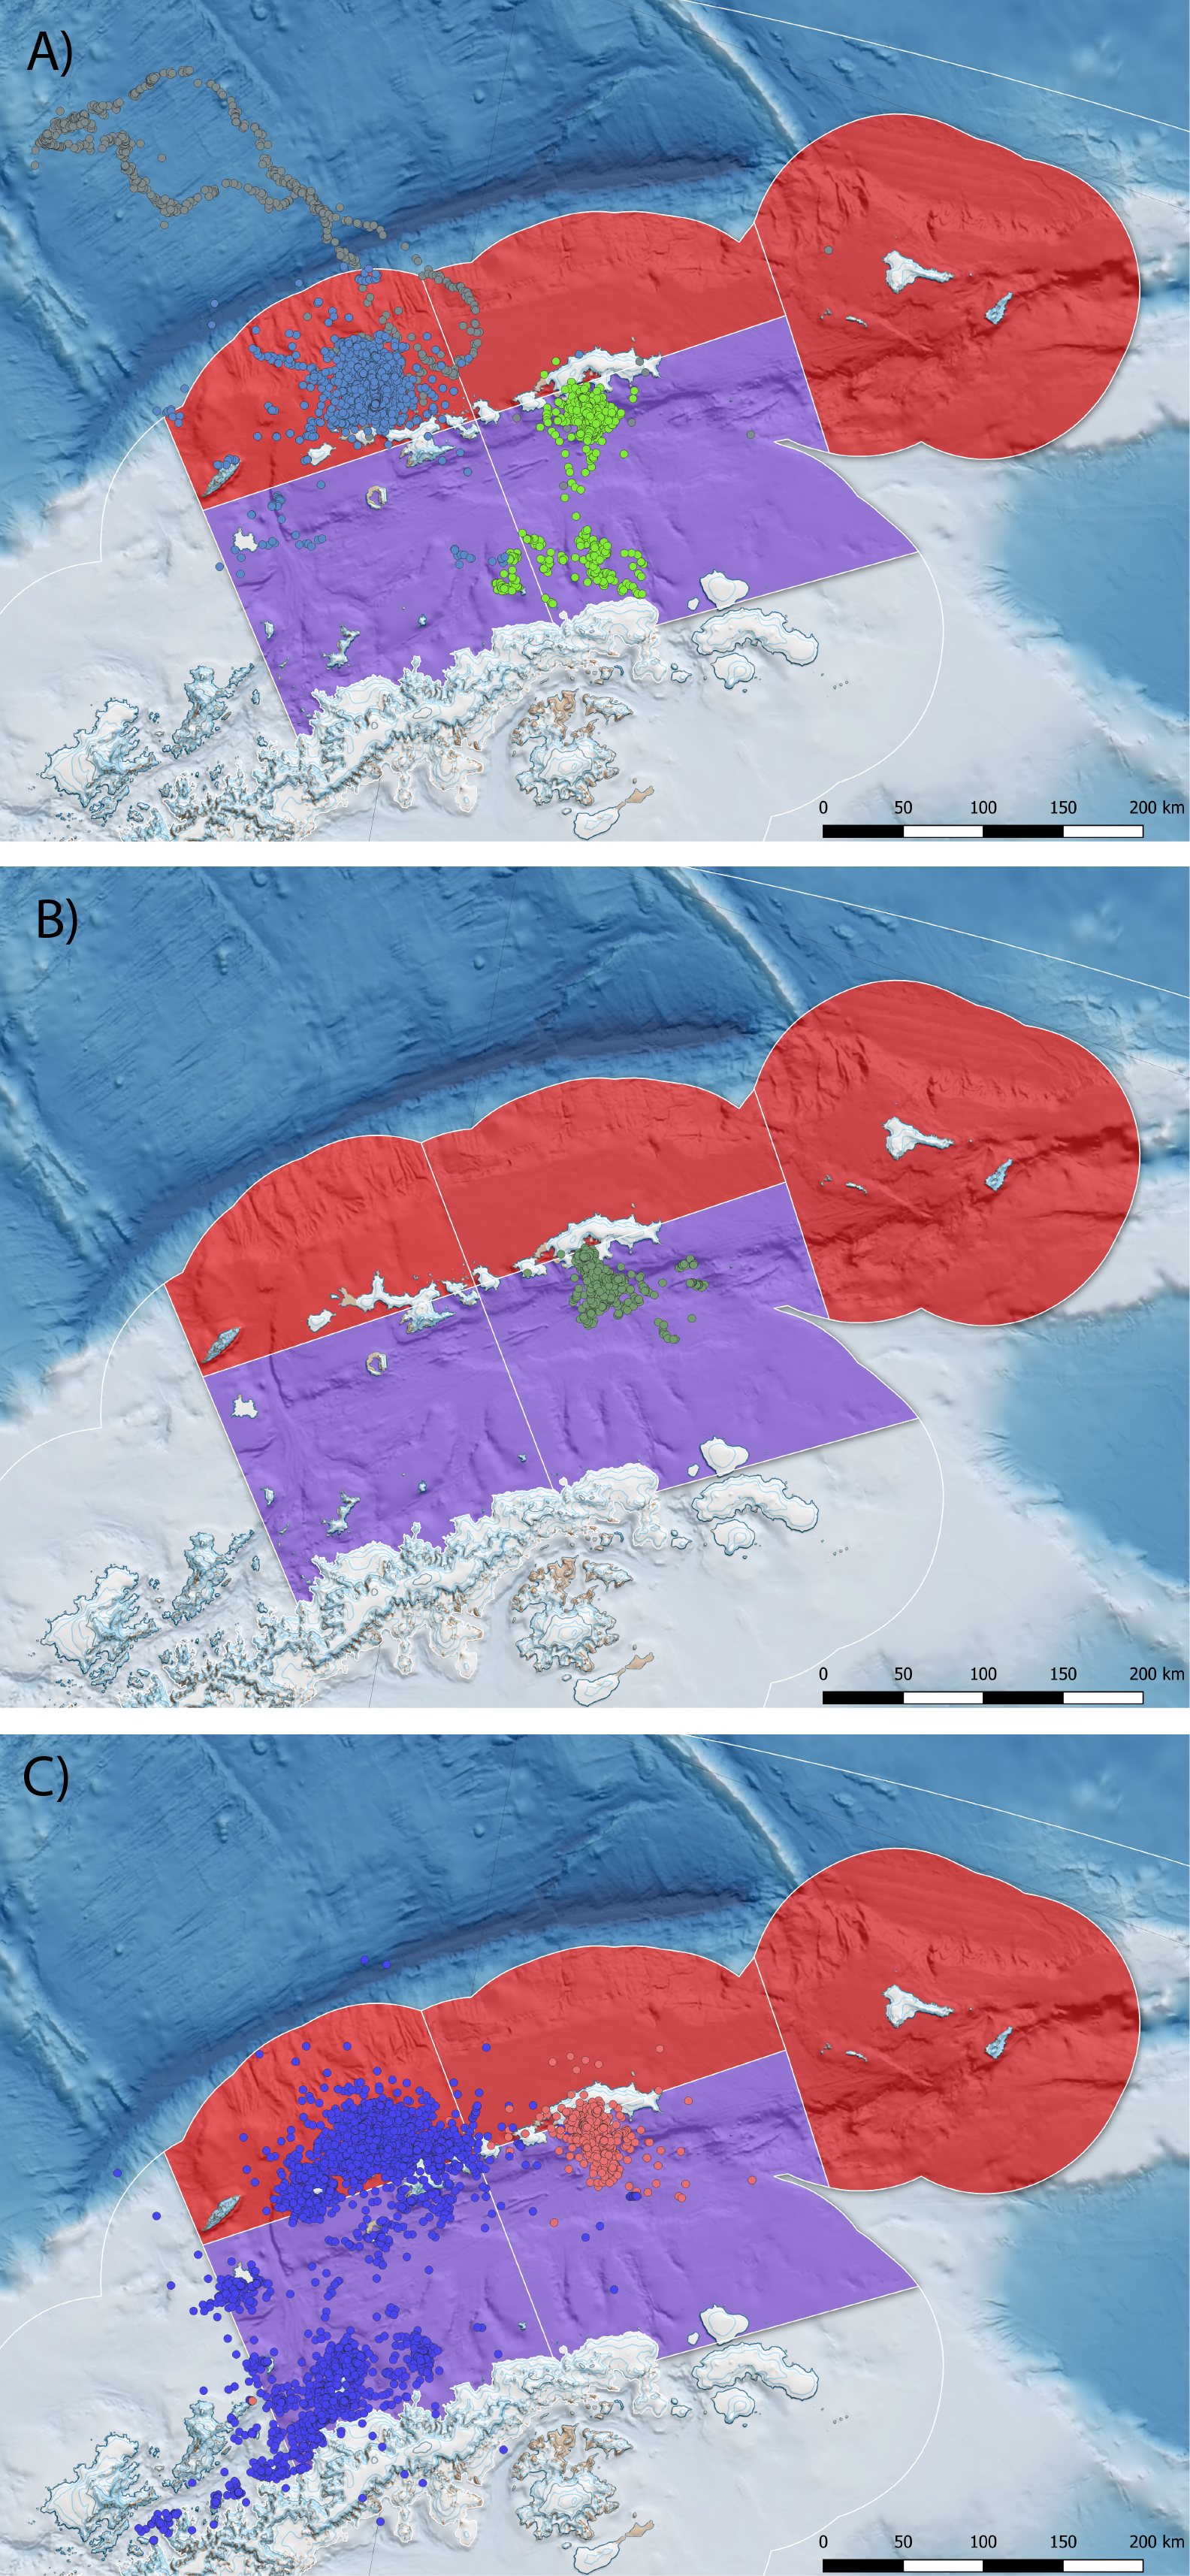
\includegraphics[width=0.65\linewidth]{./Watters EMM figures/Penguin distributions} \caption{Penguin foraging behaviour derived from available ARGOS-CLS PTT data. A) Chinstrap penguins truncated at $10^{th}$ March in line with known phenology (elongated grey track represents a single animal) B) Adélie penguins truncated to the end of January and C) Gentoo penguins until ~August, in line with known overwinter foraging behaviour. The SSMU are combined and coloured according to gSSMU (red; gSSMU 2, purple; gSSMU 1) with Chinstrap and Adélie penguin 99\% MCP home ranges occupying between 7-19\% of the gSSMU to which they were assigned.  }\label{fig:Penguin distribution plots}
\end{figure}

\begin{figure}
\includegraphics[width=0.75\linewidth]{./Watters EMM figures/Overwinter pengo distributions} \caption{A) Distribution of overwinter movement for Chinstrap penguins, relative to the gSSMU's to which they were attributed, created from telemetry data available in @Hinke2019.  B)Adélie and Chinstrap penguin movement recorded by light geolocators, highlighting the large longitudinal range both species disperse through at the end of breeding (taken from @Hinke2015).  In the original model formulation by Watters et al. 2020, the performance indices for both species are matched to gSSMU-scale estimates of LKB and LHR, but macroscale levels of ONI variability.}\label{fig:Overwinter penguin distribution plots}
\end{figure}

\begin{figure}
\includegraphics[width=1.2\linewidth]{./Watters EMM figures/Other spp distribution} \caption{The summer distribution of foraging effort by A) adult female Antarctic fur seals (adapted from telemetry data available in Hinke et al. 2017), B) migratory adult male Antarctic fur seals (adapted from Lowther et al. 2020) C) humpback whales throughout December (adapted from Johannessen et al., this meeting) and D) nonbreeding adult Adélie penguins during the breeding season (adapted from data in Oosthuizen et al., this meeting). Potential effects of competitive overlap between pygoscelid penguins and other krill dependent predators, particularly those who have increased their abundance dramatically over the preceding 40 years, should be considered when attempting to interpret variance in penguin vital rates.}\label{fig:other species plots}
\end{figure}

\begin{figure}
\includegraphics[width=1\linewidth]{./Watters EMM figures/48.1 catches in march} \caption{Daily accumulated catch (and fitted LOESS smooth curves) in Subarea 48.1 between 20$^{th}$ February and March 31$^{st}$ between A) 1990-2010 and B) 2010 to 2020. Catch in the Subarea was relatively consistent during the latter stages of penguin breeding at approximately 250tonnes/d.  However, since 2010 there has been a tendency for the fishery to increase its effort in the Subarea, starting around the middle of March. C) During this latter period, the fishery increased effort earlier on three occasions (2013, 2015 and 2016), starting before the beginning of March.}\label{fig:March Subarea 48.1 fishing plot}
\end{figure}

\bibliography{mylib.bib}


\end{document}
